\documentclass[tikz,border=2mm]{standalone}
\usepackage{pgfplots}
\pgfplotsset{compat=1.18}
\begin{document}
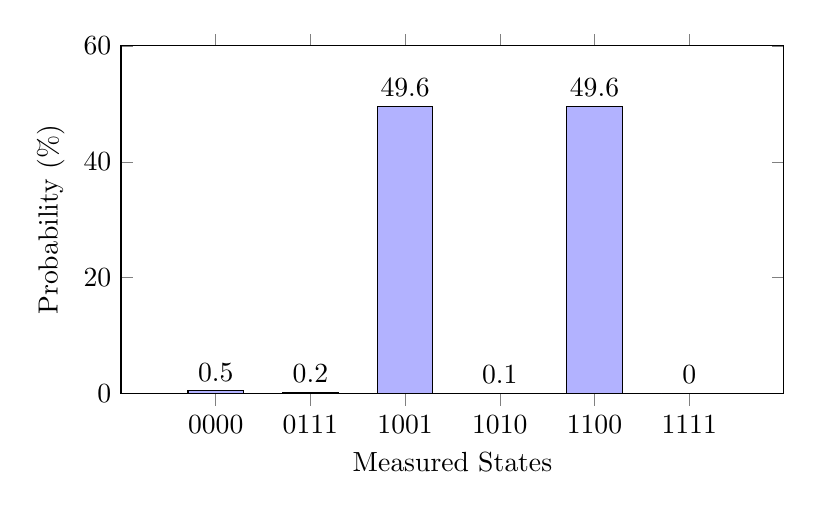
\begin{tikzpicture}
\begin{axis}[
    ybar,
    symbolic x coords={0000, 0111, 1001, 1010, 1100, 1111},
    xtick=data,
    nodes near coords,
    nodes near coords align={vertical},
    ymin=0, ymax=60,
    ylabel={Probability (\%)},
    xlabel={Measured States},
    enlarge x limits=0.2,
    bar width=20pt,
    width=10cm,
    height=6cm
]
\addplot[fill=blue!30] coordinates {(0000,0.5) (0111,0.2) (1001,49.6) (1010,0.1) (1100,49.6) (1111,0.0)};
\end{axis}
\end{tikzpicture}
\end{document}
